\chapter{Sistemi Multiagente}

\qs{}{Perché sistemi distribuiti di agenti?}

\begin{itemize}
  \item Le soluzioni centralizzate sono spesso impraticabili perché i sistemi e i dati coinvolti appartengono a organizzazioni indipendenti. 
  \item Le informazioni coinvolte sono distribuite e risiedono in sistemi informativi di grosse dimensioni e complessi sotto diversi punti di vista:
    \begin{itemize}
      \item Distribuiti geograficamente.
      \item Composti da molte parti indipendenti. 
      \item Contenuti di grandi dimensioni. 
      \item Coprono una porzione maggiore del dominio considerato.
    \end{itemize}
\end{itemize}

\paragraph{Ci sono quattro tecniche principali per affrontare la \fancyglitter{dimensione} e la \fancyglitter{complessità} di un sistema informativo:}

\begin{itemize}
  \item Modularità. 
  \item Distribuzione. 
  \item Astrazione. 
  \item Intelligenza.
\end{itemize}

\nt{L'uso di moduli distribuiti Intelligenti combinati a queste tecniche produce un approccio di \fancyglitter{intelligenza artificiale distribuita} (DAI). Gli agenti fanno parte di questo approccio.}

\dfn{Sistemi Autonomi di Agenti}{
  Per lo sviluppo di soluzioni globali e distribuite gli agenti necessitano di essere eseguiti in maniera autonoma e sviluppati indipendentemente. Gli agenti coordinano, cooperano e, eventualmente, competono per la soluzione di problemi, condividendo capacità e lavorando in parallelo. Questo porta ai sistemi Multiagente.
}

\nt{Sistemi autonomi rappresentano soluzioni modulari e riutilizzabili.}

\qs{}{Perché comunicare?}

\begin{itemize}
  \item Gli agenti operano in ambienti che contengono altri agenti.
  \item Un sistema multiagente è un sistema che contiene agenti che interagiscono tra di loro attraverso la \fancyglitter{comunicazione}. 
  \item Hanno le seguenti caratteristiche:
    \begin{itemize}
      \item Forniscono un'infrastruttura specifica per la comunicazione e l'utilizzo di protocolli di interazione. 
      \item Sono progettati per essere \fancyglitter{aperti} e \fancyglitter{distribuiti}. 
      \item Gli agenti ospitati sono \fancyglitter{autonomi}, \fancyglitter{self-interested} o \fancyglitter{cooperativi}.
    \end{itemize}
  \item Le infrastrutture includono:
    \begin{itemize}
      \item \fancyglitter{Protocolli di comunicazione:} per permettere agli agenti di comprendere i messaggi scambiati. 
      \item \fancyglitter{Protocolli di interazione:} per permettere agli agenti di svolgere conversazioni, ossia scambi strutturati di messaggi. 
    \end{itemize}
  \item Gli agenti coordinano le loro azioni e i loro comportamenti. Quest'abilità è parte della percezione (ricevere messaggi) e parte delle azioni (inviare messaggi). 
  \item La \fancyglitter{coordinazione} è una proprietà di un sistema di agenti che eseguono attività in un ambiente condiviso. 
  \item La \fancyglitter{cooperazione} è coordinazione tra agenti non antagonisti. 
  \item La \fancyglitter{negoziazione} è coordinazione tra agenti antagonisti, competitivi o self-interested.
\end{itemize}

\paragraph{Un protocollo di comunicazione potrebbe includere i seguenti tipi di messaggio:}

\begin{itemize}
  \item Proposta di esecuzione di un'azione. 
  \item Accettare una proposta. 
  \item Rifiutare una proposta. 
  \item Ritirare una proposta. 
  \item Esprimere disaccordo rispetto a una proposta. 
  \item Proporre una differente esecuzione.
\end{itemize}

\section{Agent Communication Languages}

\nt{Gli oggetti lo fanno perché devono. Gli agenti lo fanno perché vogliono.}

\subsection{Atti Comunicativi}

\dfn{Azioni Comunicative}{
  Gli agenti non possono forzare altri agenti a eseguire qualche azione (come nel paradigma object-oriented). Possono eseguire \newfancyglitter{azioni comunicative} al fine di influenzare altri agenti in modo opportuno.
}

\begin{itemize}
  \item Il linguaggio parlato umano è usato come modello per la comunicazione tra agenti. 
  \item Austin e Searle introducono la teoria nota come \fancyglitter{speech act theory} che tratta la comunicazione come azioni (requesting, informing, replying, etc.). 
  \item Gli atti comunicativi sono spiegati in termini di intenzioni degli agenti, con riferimento a beliefs, desires, intentions e altre modalità.
  \item  Un atto comunicativo ha tre aspetti:
    \begin{itemize}
      \item \fancyglitter{Locuzione:} l'atto fisico compiuto da chi parla, la produzione di enunciati grammaticali.
      \item \fancyglitter{Illocuzione:} il significato inteso dell'enunciato da parte del parlante, quello che il parlante desidera esprimere. 
      \item \fancyglitter{Perlocuzione:} l'azione che risulta dalla locuzione.
    \end{itemize}
\end{itemize}

\nt{La speech act theory usa il termine \fancyglitter{performativa} per indicare la forza illocutoria dell'enunciato.}

\paragraph{Condizioni per il successo (Austin's felicity conditions):}

\begin{itemize}
  \item Deve esistere una procedura convenzionale accettata per la performativa, le circostanze e le persone coinvolte devono essere come specificato nella procedura. 
  \item La procedura deve essere eseguita correttamente e completamente. 
  \item L'atto deve essere sincero e la comprensione deve essere completa.
\end{itemize}

\paragraph{Un Agent Communication Language (ACL):}

\begin{itemize}
  \item Fornisce agli agenti i mezzi per scambiarsi informazioni e conoscenza. 
  \item È solitamente a un livello a un livello più alto rispetto gli strumenti di comunicazione per i sistemi distribuiti, come remote procedure call o method invocation. 
  \item Tratta con proposizioni, regole, azioni. 
  \item Un messaggio descrive uno stato desiderato attraverso un linguaggio dichiarativo. 
\end{itemize}

\subsection{KQML e FIPA}

\dfn{Knowledge Sharing Effort}{
  Il Knowledge Sharing Effort (KSE) fu avviato dal DARPA intorno al 1990. L'obiettivo è sviluppare tecniche, metodologie e strumenti software per condivisione e riutilizzo della conoscenza.
}

\nt{La condivisione della conoscenza richiede la comunicazione che a sua volta richiede un linguaggio.}

\paragraph{Sviluppo le seguenti componenti:}

\begin{itemize}
  \item \fancyglitter{KQML:} un linguaggio di interazione di alto livello.
  \item \fancyglitter{KIF:} un linguaggio logico basato sulla logica del primordine, per esprimere proprietà di oggetti in una base di conoscenza. 
  \item \fancyglitter{Ontolingua:} un linguaggio per definire ontologie condivise, permettendo di dare significati uniformi su applicazioni diverse agli stessi concetti.
\end{itemize}

\paragraph{È utilizzato per dichiarare:}

\begin{itemize}
  \item Proprietà di cose.
  \item Relazioni tra cose. 
  \item Proprietà generali.
\end{itemize}

\dfn{Knowledge Query and Manipulation Language (KQML)}{
  KQML è un linguaggio di comunicazione di alto livello e indipendente da:
  \begin{itemize}
    \item Meccanismo di trasporto. 
    \item Il linguaggio in cui è espresso il contenuto. 
    \item L'ontologia utilizzata.
  \end{itemize}
}

\clm{}{}{
  \begin{itemize}
    \item Un messaggio KQML specifica il tipo di messaggio (performativa). 
    \item KQML ignora la porzione di messaggio che fa riferimento al contenuto. 
    \item La sintassi di un messaggio KQML si basa su una notazione a lista simile a quella di Lisp. 
    \item Consiste in una performativa seguita da un numero di coppie "parola chiave/valore".
  \end{itemize}
}

\paragraph{Parole chiavi riservate di KQML:}

\begin{itemize}
  \item sender: il mittente della performativa. 
  \item receiver: il destinatario della performativa. 
  \item reply-with: se il mittente si aspetta una risposta. 
  \item in-reply-to: se il mittente si aspetta una risposta. 
  \item language: il linguaggio di rappresentazione del content.
  \item ontology: l'ontologia assunta dal parametro content. 
  \item content: il contenuto del messaggio. 
\end{itemize}

\paragraph{Alcune parole performative di KQML:}

\begin{itemize}
  \item achieve: il sender vuole che il receiver esegua qualcosa. 
  \item advertise: il sender vuole una delle risposte del receiver alla domanda espressa dal content. 
  \item ask-one: il sender vuole una delle risposte del receiver alla domanda espressa dal content. 
  \item ask-all: il sender vuole tutte le risposte del receiver alla domanda espressa dal content. 
  \item reply: si comunica una risposta attesa. 
  \item sorry: il sender non può fornire una risposta più specifica. 
  \item tell: il sender informa il receiver che conosce il content.
\end{itemize}

\cor{Communication Facilitators}{
  KQML introduce una classe speciale di agenti chiamati communication facilitators che dispongono di un insieme di performative per inoltrare messaggi, trovare servizi, etc.
}

\begin{figure}[!h]
    \centering
    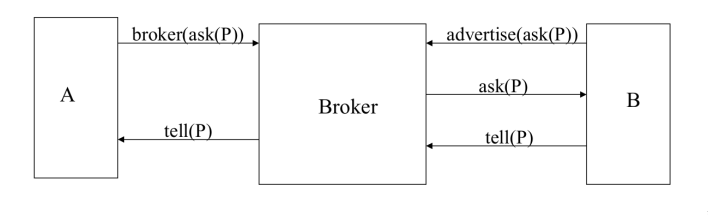
\includegraphics[scale=0.7]{04/cf.png}
  \caption{Communication Facilitators.}
\end{figure}

\cor{Semantica di KQML}{
Precondizioni, postcondizioni e condizioni di completamento descrivono lo stato degli agenti in un linguaggio basato su stati mentali espressi mediante attitudini e descrivono azioni.
}

\nt{Non è fornito un modello semantico per gli stati mentali espressi mediante attituidini.}

\dfn{FIPA ACL}{
  La Foundation for Intelligent Physical Agents (FIPA) è stata fondata con il fine di produrre degli standard per il software per agenti interagenti ed eterogenei e sistemi basati su agenti. FIPA opera attraverso una collaborazione aperta internazionale di organizzazioni associate, aziende, centri di ricerca e università. FIPA ACL è un linguaggio per comunicazione per agenti simile a KQML.
}

\paragraph{KWML vs. FIPA ACL:}

\begin{itemize}
  \item I due linguaggi sono simili alla base. 
  \item Non sono vincolati a un linguaggio per esprimere il contenuto. 
  \item La differenza principale è la semantica. 
  \item Un'altra differenza è la mancanza di primitive di tipo facilitators in FIPA ACL.
\end{itemize}


\cor{Semantica di FIPA ACL}{
  Il Semantic Language (SL) è un linguaggio formale per definire la semantica di FIPA ACL. È una logica multimodale quantificata con operatori modali. Per permettere il ragionamento su azioni, l'universo del discorso coinvolge sequenze di eventi.
}

\begin{itemize}
  \item I seguenti operatori sono introdotti per ragionare sulle azioni:
    \begin{itemize}
      \item Feasible$(a, \phi)$: $a$ può occorrere e se occorre, $\phi$ sarà vera dopo tale occorrenza. 
      \item Done$(a, \phi)$: $a$ è appena occorsa e $\phi$ è vera dopo tale occorrenza. 
      \item Agent$(i, a)$: $i$ è il solo agente che esegue l'azione $a$. 
    \end{itemize}
  \item Sulla base di beliefs, choices ed eventi viene definito il concetto di \fancyglitter{goal persistente} $PG_{i\phi}$. 
  \item L'intenzione $I_{i\phi}$ è definita come un goal persistente che impone all'agente di agire. 
  \item La semantica degli atti comunicativ è specificata come un insieme di formule $SL$ che descrivono le precondizioni di fattibilità e gli effetti razionali.
  \item \fancyglitter{Feasibility Conditions:} condizioni che devono valere per il mittente per eseguire in modo appropriato gli atti comunicativi. 
  \item \fancyglitter{Rational Effects:} gli effetti che un agente può aspettarsi che occorrano come risultato dell'esecuzione di un azione. All'agente destinatario non è richiesto di garantire che  occorra l'effetto atteso. 
  \item Per \fancyglitter{conformità} di FIPA ACL si intende che quando un agente $A$ esegue un atto comunicativo $c$, le FP$(c)$ per $A$ devono valere. I RE$(c)$ non sono garantiti e sono irrilevanti al fine della conformità.
\end{itemize}

\paragraph{Test di conformità:}

\begin{itemize}
  \item Sintattico: l'obiettivo è determinare se un agente rispetta la sintassi del linguaggio ogni volta che comunica.
      \item Semantica: l'obiettivo è determinare se un agente rispetta la semantica del linguaggio ogni volta che comunica.
\end{itemize}

\nt{Wooldridge propose un approccio basato sulla riduzione a un problema di verifica di proprietà di un programma, ma la maggior parte dei vincoli sono espressi sul mittente e questo comporta la necessità di parlare di stati mentali che non sono sempre desumibili.}

\section{Semantica Sociale per la Comunicazione}

La semantica basata su stati mentali è adeguata per sistemi di agenti cooperanti ma ha alcuni problemi per quanto riguarda i sistemi ad agenti composti da agenti eterogenei e competitivi. 

\nt{È impossibile fidarsi completamente di altri agenti o fare forti assunzioni a proposito dello stato interno degli agenti e sul loro modo di agire.}

\paragraph{L'approccio sociale:}

\begin{itemize}
  \item Considera le conseguenze sociali di eseguire un atto comunicativo. 
  \item Riconosce che la comunicazione è inerentemente pubblica e che dipende dal contesto sociale degli agenti.
\end{itemize}

\subsection{Un Buon ACL}

\paragraph{Le caratteristiche di un buon ACL:}

\begin{itemize}
  \item \fancyglitter{Formal:} chiarezza della specifica per guidare al meglio colui che realizza un sistema. 
  \item \fancyglitter{Declarative:} descrivere cosa piuttosto che come. 
  \item \fancyglitter{Verifiable:} determinare se un agente sta agendo in accordo con una data semantica. 
  \item \fancyglitter{Meaningful:} trattare la comunicazione secondo il suo significato e non come arbitrari token che devono essere ordinati in una qualche maniera.
\end{itemize}

\paragraph{Semantica per ACL basata su stati mentali e verifica:}

\begin{itemize}
  \item Rispettare un protocollo: un protocollo è rispettato se e solo se l'interazione specificata/desiderata occorre durante l'esecuzione. 
  \item Verificare un protocollo: necessità di una semantica basata su fatti osservabili.
  \item La semantica basata su stati mentali è particolarmente adatta per ragionare in modo statico sulle proprietà del protocollo e sulle politiche adottate dagli agenti. 
  \item Non è possibile fare introspezione sugli agenti perché solitamente lo stato mentale degli agenti non è accessibile.
\end{itemize}

\paragraph{È necessaria una semantica che sia:}

\begin{itemize}
  \item Indipendente dagli stati mentali dei partecipanti.
  \item Verificabile sia da un partecipante sia da una terza parte che deve monitorare l'interazione. 
  \item Possibile rendere osservabile la violazione di una specifica da parte di un partecipante all'interazione. 
\end{itemize}

\clm{}{}{
  \begin{itemize}
    \item L'approccio è basato sui pratical commitment tra agenti: un agente (il debtor) si impegna verso un altro agente (il creditor) a rendere vero un qualche fatto o a eseguire una qualche azione. 
    \item I vari atti illocutori possono essere visti in termini di commitment sociali che i partecipanti creano.
  \end{itemize}
}

\nt{La comunicazione nell'approccio sociale è inerentemente pubblica.}

\paragraph{Commitment (per Castelfranchi):}

\begin{itemize}
  \item Un commitment sociale ha natura normativa e genera diritti. 
  \item Cancellare o ritirare un commitment viola un'obbligazione non implica un'informazione verso la contropare, ma frustra delle aspettative e dei diritti che l'agente ha creato.
\end{itemize}

\paragraph{Commitment (per Singh):}

\begin{itemize}
  \item Include una nozione di \fancyglitter{contesto sociale} nella definizione di commitment (il team in cui l'agente partecipa e in cui comunica). 
  \item Permette \fancyglitter{metacommitment} per catturare un'ampia varietà di relazioni legali e sociali in un unico framework. 
  \item Il comportamento degli agenti è influenzato dai commitment perché l'assunzione è che gli agenti rispettino gli impegni presi. 
  \item I commitment sono manipolabili dagli agenti.
\end{itemize}

\begin{figure}[!h]
    \centering
    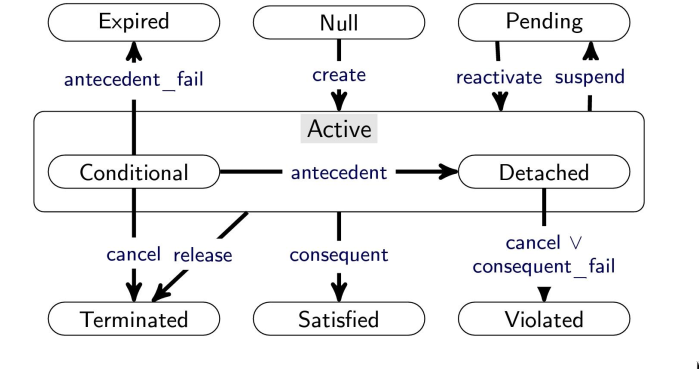
\includegraphics[scale=0.5]{04/singh.png}
  \caption{Ciclo di vita dei commitment per Singh.}
\end{figure}

\section{Protocolli di Interazione}

\begin{itemize}
  \item Gli agenti non possono prendere parte a un dialogo semplicemente scambiandosi messaggi ACL. 
  \item L'analisi di numerose conversazioni umane mostra che sono presenti dei pattern ricorrenti nelle conversazioni. 
  \item La semantica mentalistica per gli atti comunicativi è troppo complessa per determinare una possibile risposta a un messaggio. 
  \item Un agente ha bisogno di \fancyglitter{conversation policies}/\fancyglitter{Protocolli di interazione}. 
  \item In generale i protocolli specificano il contenuto della comunicazione.
\end{itemize}

\begin{figure}[!h]
    \centering
    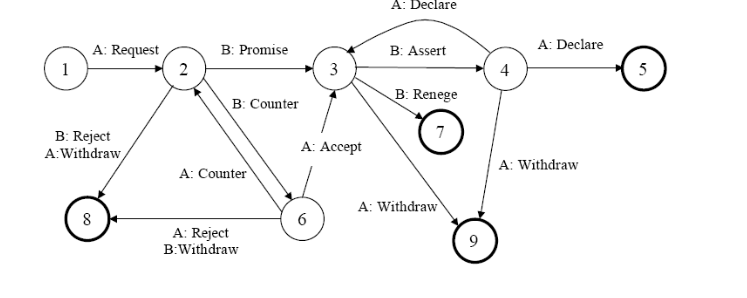
\includegraphics[scale=0.5]{04/protocollo.png}
  \caption{Protocollo rappresentato come DFA.}
\end{figure}

\dfn{Contract Net Protocol (task sharing)}{
  Un protocollo per realizzare sistemi di agenti cooperanti. È modellato sul meccanismo di contrattazione utilizzato per governare gli scambi di merci e servizi. Un agente che desidera che un task sia risolto viene chiamato manager (initiator) e gli agenti che potrebbero risolvere il task sono chiamati contractors (participants).
}

\paragraph{Un agente ha un goal e realizza che:}

\begin{itemize}
  \item O non è in grado di soddisfarlo in autonomia, ma non ne ha le capacità. 
  \item O preferirebbe non soddisfarlo in autonomia, per ottenere una soluzione migliore.
\end{itemize}

\paragraph{Task Sharing:}

\begin{itemize}
  \item Manager: 
    \begin{itemize}
      \item Annuncia un task che necessita di essere risolto. 
      \item Riceve e valuta le offerte dei possibili contractors. 
      \item Sceglie un contractor e lo informa. 
      \item Riceve il risultato.
    \end{itemize}
  \item Contractor: 
    \begin{itemize}
      \item Ricever gli annunci di task dal manager. 
      \item Valuta il task. 
      \item Risponde declinando o facendo un'offerta (bidding). 
      \item Esegue il task se l'offerta è stata accettata. 
      \item Riporta il risultato (expediting).
    \end{itemize}
  \item Un contractor per un task può agire a sua volta da manager sollecitando l'aiuto di altri agenti per risolvere parte di quel task. 
  \item Una deadline può essere fissata per effettuare offerte da parte dei contractors.
\end{itemize}

\subsection{Protocolli a commitment}


\begin{itemize}
  \item I protocolli possono essere specificati come un insieme di commitment piuttosto che come DFA. 
  \item Gli agenti giocano ruoli diversi nella società e i ruoli definiscono l'associazione con gli impegni sociali. 
  \item In generale, gli agenti possono gestire i propri impegni manipolandoli o cancellandoli. 
  \item Poiché i requisiti di un protocollo vengono espressi solamente attraverso commitment, gli agenti possono essere conformi sulla base della loro comunicazione. 
 \item L'idea è di catturare la relazione "count-as" che descrive il significato dell'azione. 
    \item Il solo vincolo che un protocollo a commitment deve soddisfare per avere successo è che tutti i componenti siano discharged. 

\end{itemize}

\dfn{Run del Protocollo a Commitment}{
  Una run del protocollo a commitment è una sequemza finita di azioni che portano in uno stato in cui tutti i commitment sono discharged, ossia non ci siano commitment pendenti.
}

\clm{}{}{
  \begin{itemize}
    \item Data la precedente specifica delle azioni, si può costruire delle sequenze che permettono di raggiungere uno stato in cui non ci siano commitment pendenti. 
    \item Verifica: data una sequenza di azioni eseguite dagli agenti, si può verificare se essa sia o non sia una sequenza ammessa dal protocollo.
  \end{itemize}
}

\subsection{Information Protocols}

\nt{Proposta recente di Singh, presentati nel 2011.}

\paragraph{Proprietà dei partecipanti all'interazione:}

\begin{itemize}
  \item Autonomia. 
  \item Miopia:
    \begin{itemize}
      \item Tutte le scelte devono essere locali. 
      \item La correttezza non deve basarsi su interazioni future.
    \end{itemize}
  \item Eterogeneità:
    \begin{itemize}
      \item Stato locale:
        \begin{itemize}
          \item Pubblico od osservabile. 
          \item Deve essere rivelato, per correttezza.
        \end{itemize}
      \item Stato interno: 
        \begin{itemize}
          \item Privato. 
          \item Non deve mai essere rivelato, per evitare falsi accoppiamenti.
        \end{itemize}
    \end{itemize}
  \item Rappresentazione condivisa dello stato locale: 
    \begin{itemize}
      \item Eseguita tramite messaggistica.
    \end{itemize}
\end{itemize}

\dfn{Blindingly Simple Protocol Language (BSPL)}{
  Ci sono due notazioni sintattiche:
  \begin{itemize}
    \item Dichiarare uno schema di messaggio come protocollo atomico. 
    \item Dichiarare un protocollo come un insieme di riferimenti a protocolli.
  \end{itemize}
  I parametri sono centrali:
  \begin{itemize}
    \item Base per esprimere il significato in termini di binding. 
    \item Specifica non ambigua. 
    \item Catturano: 
      \begin{itemize}
        \item La progressione della conoscenza di un ruolo. 
        \item La \fancyglitter{completness} di un \fancyglitter{enactment} di protocollo. 
        \item L'unicità degli enactment tramite chiavi (key).
      \end{itemize}
  \end{itemize}
}

\cor{Key}{
  Le Key: 
  \begin{itemize}
    \item Tutti i parametri chiave insieme formano una chiave. 
    \item Almeno un parametro chiave per protocollo. 
    \item Almeno un parametro chiave in comune durante messaggi e riferimenti ad altri protocolli. 
    \item La chiave di un protocollo fornisce una base per l'unicità dei suoi enactment.
  \end{itemize}
}

\paragraph{Ornamenti dei parametri:}

\begin{itemize}
  \item in: informazioni che devono essere fornite per istanziare un protocollo. 
  \item out: informazioni generate dalle istanze del protocollo. 
  \item nil: informazioni assenti dall'istanza di protocollo.
\end{itemize}

\paragraph{Idee principali dei protocolli BSPL:}
\begin{itemize}
  \item Dichiarativo: 
    \begin{itemize}
      \item Nessun flusso o stato di controllo.
    \end{itemize}
  \item Basato sulle informazioni: 
    \begin{itemize}
      \item Specifica la computazione dell'informazione distribuita: 
        \begin{itemize}
          \item La specifica di un messaggio è esso stesso un protocollo.
        \end{itemize}
      \item Specificano tramite parametri. 
    \end{itemize}
  \item La causalità è esplicita:
    \begin{itemize}
      \item I messaggi che un agente può inviare dipendono da ciò che conosce.
    \end{itemize}
  \item Integrity: 
    \begin{itemize}
      \item L'agente invia solo messaggi che preservano la coerenza delle informazioni. 
      \item Tramite vincoli di chiave.
    \end{itemize}
  \item Messaggistica sincrona. 
  \item Non richiede alcun ordinamento dall'infrastruttura. 
  \item Composizione e verifica.
  
\end{itemize}

\qs{}{Quando un messaggio è valido? Quale effetto ha sulla conoscenza locale di un ruolo?}

\begin{itemize}
  \item Out: crea e trasmette conoscenza. 
  \item In: trasmette conoscenza. 
  \item Le ripetizioni attraverso percorsi multipli sono innocue e superflue.
\end{itemize}


\begin{figure}[!h]
    \centering
    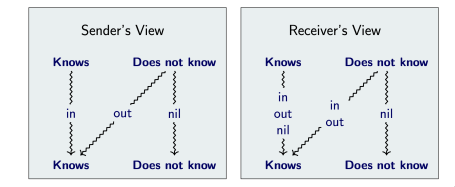
\includegraphics[scale=0.7]{04/inoutnil.png}
  \caption{Schema di BSPL.}
\end{figure}

\paragraph{Struttura causale come vincoli temporali:}

\begin{itemize}
  \item \fancyglitter{Ricezione:} se un messaggio viene ricevuto, è stato precedentemente inviato. 
  \item \fancyglitter{Trasmissione delle informazioni:} 
    \begin{itemize}
      \item I parametri "in" si verificano prima del messaggio. 
      \item I parametri "out" si verificano simultaneamente al messaggio.
    \end{itemize}
  \item \fancyglitter{Ricezione delle informazioni:} qualsiasi parametro "in" o "out" si verifica prima o simultaneamente al messaggio.
    
  \item \fancyglitter{Minimalità delle informazioni:} se un ruolo osserva un parametro deve essere simultaneamente a un messaggio inviato o ricevuto. 
  \item \fancyglitter{Ordinamento:} se un ruolo invia due messaggi li osserva in ordine.
\end{itemize}

\paragraph{Implementazione di BSPL:}


\begin{itemize}
  \item Per ogni ruolo: 
    \begin{itemize}
      \item Per ogni messaggio che si invia o che si riceve: 
        \begin{itemize}
          \item Mantieni una relazione locale dello stesso schema del messaggio.
        \end{itemize}
    \end{itemize}
  \item Ricevi e archivia ogni messaggio ricevuto: 
    \begin{itemize}
      \item Che non sia un duplicato. 
      \item Che i vincoli di integrità siano rispettati. 
      \item Cancella le sessioni scadute. 
    \end{itemize}
  \item Invia qualsiasi messaggio univoco purché:
    \begin{itemize}
      \item I binding dei parametri concordino con i binding precedenti per le stesse chiavi per i parametri "in". 
      \item Non esistano binding per i parametri "out" e "nil".
    \end{itemize}
\end{itemize}

\nt{Ogni interazione è caratterizzata solo in termini di informazione: causalità esplicita, chiavi, integrità, immutabilità.}

\subsection{Modelli di Coordinazione}

\dfn{Blackboard}{
  Un approccio alternativo alla progettazione, realizzazione e gestione di sistemi multiagente. È basato su modelli di coordinazione che ad alto livello sono finalizzati a regolare il comportamento delle diverse componenti di un sistema. Un Blackboard system è un approccio basato sull'architettura a lavagna dove una base di conoscenza comune è iterativamente aggiornata da sorgenti di conoscenza, partendo da una specifica di un problema alla soluzione. 
}

\nt{Ogni sorgente di conoscenza aggiorna la blackboard con una soluzione parziale.}

\dfn{Norme}{
  Le norme e le leggi sociali sono uno dei meccanismi più diffusi per coordinare le attività. Una norma esprime uno schema di comportamento atteso. Le norme possono essere enforced o meno e possono emergere dal sistema o essere progettate.
}
